% ============================================================================================================
\chapter{Comparaison des stratégies}\label{ch:strategies}
% ============================================================================================================

\section{Cinq stratégies, cinq définitions explicites}

Chaque stratégie est définie par un objectif et des contraintes, posés avant le calcul :
\begin{description}
\item[S1 Protection sociale et pouvoir d'achat] maximiser le niveau de vie des 30 \% les plus modestes et le revenu
disponible réel ; dette à 10 et 20 ans non accrue, chômage non accru, aucun décile ne perd plus de 0,5 \% ; par
définition, aucune réduction de droits sociaux ni de dépenses de santé, d'éducation et d'emploi public.
\item[S2 Compétitivité et emploi] minimiser le chômage à 10 ans ; dette non accrue, exportations et PIB non réduits,
niveau de vie des modestes non réduit de plus de 0,5 \%, aucun décile ne perd plus de 1 \%.
\item[S3 Productivité et transformation] maximiser le PIB à 15 ans, avec une productivité par emploi en hausse d'au
moins 0,5 \%, sans baisse de l'emploi ni de l'investissement ; dette à 15 ans non accrue.
\item[S4 Redressement budgétaire accéléré] minimiser la dette à 10 ans ; chômage accru de 0,5 point au plus, PIB réduit
de 1 \% au plus, niveau de vie des modestes réduit de 1 \% au plus, aucun décile ne perd plus de 1,5 \%.
\item[S5 Optimisation globale] maximiser le minimum des huit critères normalisés (sans pondération) ; aucun décile ne
perd plus de 1 \%.
\end{description}
Toutes sont limitées à huit leviers, dans le périmètre principal (niveaux de preuve A et B). Le
tableau~\ref{tab:strat} en donne la composition et la prévision du métamodèle.

\begin{table}[htbp]\centering\scriptsize
\caption{Composition des stratégies (écart à la situation actuelle) et prévision du métamodèle en 2037.}\label{tab:strat}
\tabfit{../tables/strategies_principal.tex}
\end{table}

\section{Vérification par le modèle complet}

Les cinq stratégies et les cinq programmes de la v0.6 ont été simulés avec le modèle complet v0.7 (microsimulation,
zone euro, comportements). Le tableau~\ref{tab:horizons} donne les effets à 5, 10, 15 et 20 ans et la
figure~\ref{fig:traj} les trajectoires.

\begin{figure}[htbp]\centering
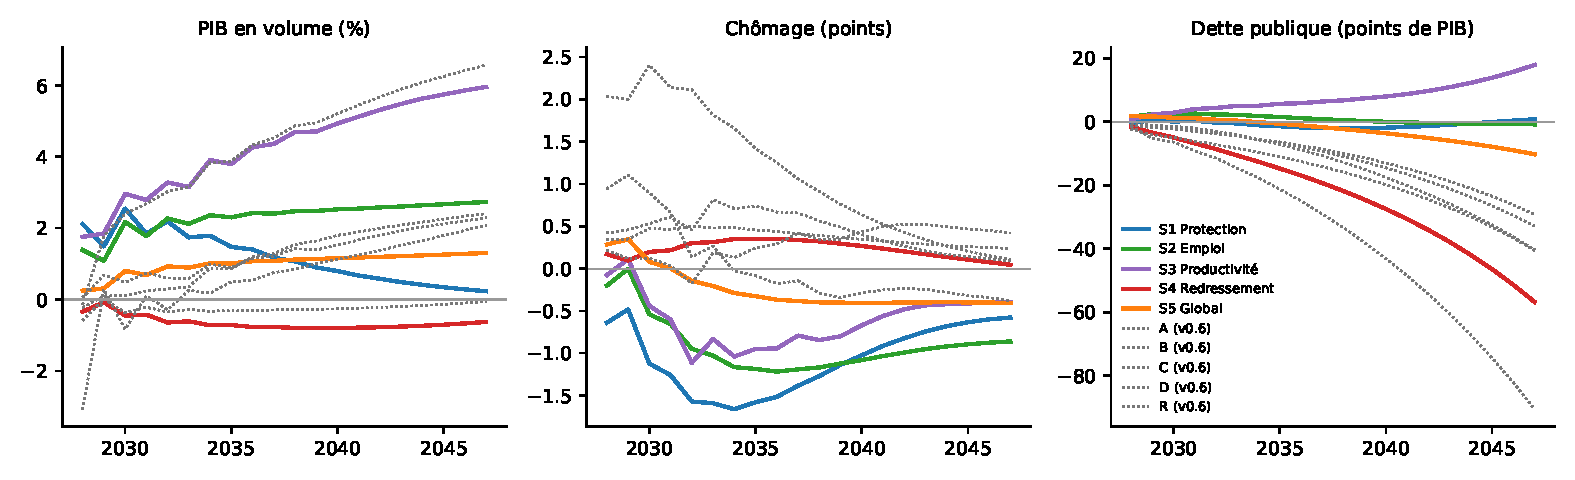
\includegraphics[width=\linewidth]{strategies_trajectoires.pdf}
\caption{Trajectoires des programmes (écarts à la référence). Traits pleins : stratégies de la phase 3 ; pointillés :
programmes de la v0.6.}\label{fig:traj}
\end{figure}

\begin{longtable}{llrrrrr}\caption{Effets des programmes à 5, 10, 15 et 20 ans (modèle complet v0.7, comportements centraux, écarts à la référence). Dernière colonne : prévision du métamodèle à 10 ans.}\label{tab:horizons}\\ \toprule Programme & Indicateur & 2032 & 2037 & 2042 & 2047 & Métam. 2037\\ \midrule\endfirsthead\toprule Programme & Indicateur & 2032 & 2037 & 2042 & 2047 & Métam.\\ \midrule\endhead
S1 Protection & PIB (\%) & $+2{,}19$ & $+1{,}17$ & $+0{,}58$ & $+0{,}23$ & $+1{,}09$\\
 & Emploi (milliers) & $+738$ & $+677$ & $+484$ & $+398$ & $+628$\\
 & Chômage (pt) & $-1{,}57$ & $-1{,}39$ & $-0{,}82$ & $-0{,}58$ & $-1{,}25$\\
 & RDB réel (\%) & $+5{,}82$ & $+6{,}39$ & $+6{,}93$ & $+7{,}41$ & $+5{,}52$\\
 & Solde (pt) & $-0{,}56$ & $-0{,}54$ & $-0{,}76$ & $-0{,}89$ & $-0{,}41$\\
 & Dette (pt) & $-0{,}3$ & $-1{,}9$ & $-1{,}3$ & $+0{,}8$ & $-1{,}8$\\
\addlinespace
S2 Emploi & PIB (\%) & $+2{,}27$ & $+2{,}41$ & $+2{,}58$ & $+2{,}73$ & $+2{,}36$\\
 & Emploi (milliers) & $+520$ & $+604$ & $+536$ & $+487$ & $+587$\\
 & Chômage (pt) & $-0{,}95$ & $-1{,}19$ & $-0{,}99$ & $-0{,}86$ & $-1{,}15$\\
 & RDB réel (\%) & $+2{,}06$ & $+2{,}76$ & $+3{,}49$ & $+4{,}11$ & $+2{,}60$\\
 & Solde (pt) & $-0{,}57$ & $-0{,}44$ & $-0{,}52$ & $-0{,}63$ & $-0{,}32$\\
 & Dette (pt) & $+2{,}3$ & $+0{,}8$ & $-0{,}4$ & $-0{,}8$ & $+0{,}0$\\
\addlinespace
S3 Productivité & PIB (\%) & $+3{,}28$ & $+4{,}36$ & $+5{,}31$ & $+5{,}96$ & $+4{,}93$\\
 & Emploi (milliers) & $+773$ & $+1139$ & $+1334$ & $+1466$ & $+1327$\\
 & Chômage (pt) & $-1{,}12$ & $-0{,}79$ & $-0{,}48$ & $-0{,}40$ & $-0{,}51$\\
 & RDB réel (\%) & $+3{,}64$ & $+5{,}19$ & $+5{,}99$ & $+6{,}54$ & $+4{,}91$\\
 & Solde (pt) & $-1{,}35$ & $-1{,}46$ & $-1{,}74$ & $-2{,}79$ & $-0{,}74$\\
 & Dette (pt) & $+4{,}3$ & $+6{,}4$ & $+9{,}7$ & $+17{,}9$ & $+2{,}4$\\
\addlinespace
S4 Redressement & PIB (\%) & $-0{,}64$ & $-0{,}77$ & $-0{,}78$ & $-0{,}63$ & $-0{,}76$\\
 & Emploi (milliers) & $-102$ & $-115$ & $-69$ & $-15$ & $-111$\\
 & Chômage (pt) & $+0{,}30$ & $+0{,}34$ & $+0{,}20$ & $+0{,}05$ & $+0{,}33$\\
 & RDB réel (\%) & $-1{,}98$ & $-2{,}01$ & $-1{,}96$ & $-1{,}80$ & $-1{,}93$\\
 & Solde (pt) & $+2{,}26$ & $+2{,}91$ & $+4{,}18$ & $+6{,}45$ & $+3{,}02$\\
 & Dette (pt) & $-8{,}6$ & $-19{,}3$ & $-34{,}1$ & $-56{,}8$ & $-20{,}0$\\
\addlinespace
S5 Global & PIB (\%) & $+0{,}93$ & $+1{,}08$ & $+1{,}20$ & $+1{,}30$ & $+1{,}07$\\
 & Emploi (milliers) & $+157$ & $+239$ & $+245$ & $+245$ & $+227$\\
 & Chômage (pt) & $-0{,}15$ & $-0{,}38$ & $-0{,}40$ & $-0{,}41$ & $-0{,}35$\\
 & RDB réel (\%) & $+1{,}00$ & $+1{,}18$ & $+1{,}42$ & $+1{,}69$ & $+1{,}38$\\
 & Solde (pt) & $+0{,}17$ & $+0{,}38$ & $+0{,}60$ & $+1{,}06$ & $+0{,}54$\\
 & Dette (pt) & $+0{,}6$ & $-1{,}7$ & $-5{,}2$ & $-10{,}3$ & $-3{,}5$\\
\addlinespace
A (v0.6) & PIB (\%) & $-0{,}35$ & $-0{,}29$ & $-0{,}22$ & $-0{,}06$ & \\
 & Emploi (milliers) & $-77$ & $-47$ & $-10$ & $+14$ & \\
 & Chômage (pt) & $+0{,}50$ & $+0{,}41$ & $+0{,}31$ & $+0{,}24$ & \\
 & RDB réel (\%) & $-0{,}85$ & $-0{,}98$ & $-1{,}08$ & $-1{,}13$ & \\
 & Solde (pt) & $+1{,}44$ & $+2{,}03$ & $+3{,}02$ & $+4{,}71$ & \\
 & Dette (pt) & $-7{,}2$ & $-14{,}2$ & $-24{,}5$ & $-40{,}5$ & \\
\addlinespace
B (v0.6) & PIB (\%) & $+3{,}02$ & $+4{,}52$ & $+5{,}68$ & $+6{,}57$ & \\
 & Emploi (milliers) & $+97$ & $+666$ & $+1001$ & $+1213$ & \\
 & Chômage (pt) & $+0{,}14$ & $-0{,}15$ & $-0{,}24$ & $-0{,}38$ & \\
 & RDB réel (\%) & $-0{,}43$ & $+0{,}75$ & $+1{,}30$ & $+1{,}82$ & \\
 & Solde (pt) & $+0{,}76$ & $+1{,}56$ & $+2{,}78$ & $+4{,}43$ & \\
 & Dette (pt) & $-3{,}1$ & $-10{,}7$ & $-22{,}9$ & $-40{,}3$ & \\
\addlinespace
C (v0.6) & PIB (\%) & $+0{,}60$ & $+1{,}22$ & $+1{,}80$ & $+2{,}29$ & \\
 & Emploi (milliers) & $+240$ & $+506$ & $+769$ & $+970$ & \\
 & Chômage (pt) & $-0{,}18$ & $+0{,}42$ & $+0{,}53$ & $+0{,}42$ & \\
 & RDB réel (\%) & $+0{,}45$ & $+1{,}13$ & $+1{,}15$ & $+1{,}20$ & \\
 & Solde (pt) & $+0{,}84$ & $+1{,}19$ & $+2{,}21$ & $+3{,}66$ & \\
 & Dette (pt) & $-3{,}8$ & $-8{,}6$ & $-16{,}7$ & $-29{,}2$ & \\
\addlinespace
D (v0.6) & PIB (\%) & $-0{,}29$ & $+0{,}75$ & $+1{,}38$ & $+2{,}09$ & \\
 & Emploi (milliers) & $-683$ & $-327$ & $-112$ & $-1$ & \\
 & Chômage (pt) & $+2{,}11$ & $+1{,}06$ & $+0{,}43$ & $+0{,}10$ & \\
 & RDB réel (\%) & $-4{,}97$ & $-4{,}93$ & $-4{,}92$ & $-4{,}87$ & \\
 & Solde (pt) & $+3{,}29$ & $+4{,}82$ & $+6{,}92$ & $+10{,}12$ & \\
 & Dette (pt) & $-11{,}5$ & $-29{,}1$ & $-54{,}3$ & $-90{,}5$ & \\
\addlinespace
R (v0.6) & PIB (\%) & $+0{,}30$ & $+1{,}29$ & $+2{,}00$ & $+2{,}41$ & \\
 & Emploi (milliers) & $-12$ & $+247$ & $+493$ & $+587$ & \\
 & Chômage (pt) & $+0{,}45$ & $+0{,}66$ & $+0{,}26$ & $+0{,}09$ & \\
 & RDB réel (\%) & $-0{,}91$ & $-0{,}20$ & $+0{,}11$ & $+0{,}31$ & \\
 & Solde (pt) & $+1{,}05$ & $+1{,}49$ & $+2{,}47$ & $+3{,}85$ & \\
 & Dette (pt) & $-3{,}7$ & $-9{,}4$ & $-18{,}8$ & $-32{,}8$ & \\\bottomrule\end{longtable}

\begin{resultat}[Ce que montre la vérification]
\begin{itemize}
\item \textbf{Le métamodèle est fiable pour S1, S2, S4 et S5} : en 2037, l'écart au modèle complet est inférieur à
0,1 point de PIB et 0,15 point de chômage ; il atteint 0,7 à 1,8 point de dette (le métamodèle est un peu optimiste
pour S2 et S5).
\item \textbf{Il ne l'est pas pour S3}, qui combine sept mesures d'offre ou de soutien à l'activité : le modèle
complet donne un PIB plus faible (+4,4 \% au lieu de +4,9 \% en 2037) et surtout une dette nettement plus élevée
(+6,4 points en 2037, +9,7 en 2042, +18 en 2047, au lieu de l'équilibre visé en 2042). Les effets des mesures d'offre
ne s'additionnent pas : elles passent toutes par le PIB potentiel et la fermeture, et leurs recettes induites se
recouvrent. C'est une interaction importante, que seul le modèle complet révèle.
\item \textbf{Coûts de transition et bénéfices de long terme diffèrent} : S2 et S3 accroissent la dette les premières
années (+2,3 et +4,3 points en 2032) ; S2 devient favorable à la dette après 2040, S3 ne le devient pas. S1 est presque
neutre pour la dette sur toute la période. S4 réduit la dette de 19 points en 2037 et de 57 points en 2047, au prix
d'un PIB inférieur de 0,8 \% et d'un chômage plus élevé de 0,3 point en 2037, effet qui s'estompe ensuite.
\end{itemize}
\end{resultat}

\section{Comparaison avec les programmes de la v0.6}

Les programmes A, B, C, D et R de la v0.6, simulés avec la v0.7, conservent leur hiérarchie budgétaire (D réduit le
plus la dette : $-29$ points en 2037 ; A $-14$ ; B $-11$ ; R $-9$ ; C $-9$). Leurs effets sur l'activité changent : B,
fondé sur la durée du travail et l'âge légal, augmente le PIB de 4,5 \% en 2037 en v0.7. S4 réduit davantage la dette
que A, B, C et R à horizon 10 ans ($-19$ points), au prix d'une baisse du PIB plus marquée que A ($-0{,}8$ \% contre
$-0{,}3$ \%) ; il est dominé par D pour la dette, mais D augmente le chômage d'un point en 2037 et fait perdre de 0,8 à
6,4 \% de niveau de vie à tous les déciles.

% ============================================================================================================
\chapter{Gagnants et perdants}\label{ch:gagnants}
% ============================================================================================================

\begin{limites}[Portée du calcul]
Les gagnants et perdants sont calculés par la microsimulation, sur les revenus de l'année de base et avant les effets
macroéconomiques (emploi, salaires, prix). Les mesures qui ne touchent pas directement le revenu des ménages ne sont
pas imputées : impôt sur les sociétés, impôts de production, cotisations employeurs, droits de succession,
investissement et dépenses publiques. Leur coût pour les actionnaires, les héritiers ou les usagers des services
publics n'apparaît donc pas ici. Les montants sont en euros par unité de consommation et par an.
\end{limites}

\begin{figure}[htbp]\centering
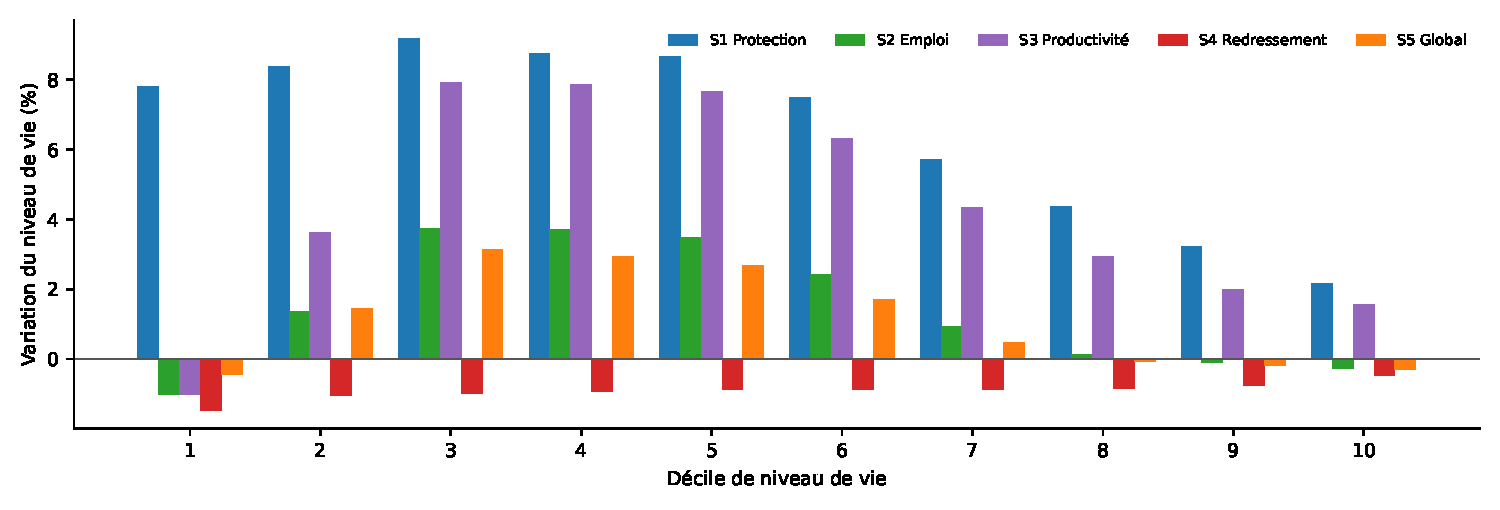
\includegraphics[width=\linewidth]{deciles.pdf}
\caption{Variation du niveau de vie par décile (microsimulation statique).}\label{fig:deciles}
\end{figure}

\paragraph{Par décile.} S1 augmente le niveau de vie de tous les déciles, de 7,8 \% (426 € par unité de consommation)
pour le premier décile à 2,2 \% pour le dernier ; le taux de pauvreté (seuil fixe) passe de 17,3 \% à 13,8 \% et
l'indice de Gini de 0,349 à 0,334. S2, S3 et S5 profitent surtout aux déciles 2 à 7 (prime d'activité) ; le premier
décile perd légèrement (de 0,5 à 1 \%, environ 25 à 55 € par unité de consommation) du fait de la baisse des aides au
logement et des allocations chômage, et, pour S2 et S5, les deux derniers déciles perdent jusqu'à 0,3 \%. S4 fait perdre de 0,5 à
1,5 \% à tous les déciles (de 80 € pour le premier à 340 € pour le dernier), et augmente la pauvreté de 0,3 point.

\paragraph{Par génération.} S4 est la stratégie la plus défavorable aux plus âgés : $-1{,}8$ \% pour les ménages dont la
personne de référence a 75 ans ou plus, $-1{,}3$ \% pour les 60-74 ans, du fait de la sous-indexation des pensions.
S1, S2, S3 et S5 profitent surtout aux moins de 60 ans. S3 relève l'âge légal de deux ans, ce qui pèse sur les
générations nées après 1965 ; cette perte (retraite plus tardive) n'est pas mesurée par la microsimulation.

\begin{table}[htbp]\centering\scriptsize
\caption{Variation du niveau de vie par âge de la personne de référence (€ par unité de consommation et par an).}
\tabfit{../tables/groupes_age.tex}
\end{table}

\paragraph{Par catégorie sociale.} Les ouvriers et les employés sont les principaux gagnants de S1, S2, S3 et S5 (de
+2,5 à +9,7 \%). Les inactifs non retraités (étudiants, personnes au foyer) perdent dans S2 ($-3{,}3$ \%) et S3
($-1{,}4$ \%) : ce sont les principaux bénéficiaires des aides au logement. Les retraités perdent dans S4 ($-1{,}8$ \%).

\begin{table}[htbp]\centering\scriptsize
\caption{Variation du niveau de vie par catégorie sociale de la personne de référence (€ par unité de consommation et
par an).}
\tabfit{../tables/groupes_csp.tex}
\end{table}

\paragraph{Par configuration familiale.} Les familles monoparentales et les couples avec trois enfants ou plus sont
les principaux gagnants des stratégies qui augmentent la prime d'activité, le RSA ou les allocations familiales.

\begin{table}[htbp]\centering\scriptsize
\caption{Variation du niveau de vie par configuration familiale (€ par unité de consommation et par an).}
\tabfit{../tables/groupes_famille.tex}
\end{table}

\paragraph{Par territoire.} Les écarts entre régions sont faibles comparés aux écarts entre catégories ; ils
reflètent la composition sociale des régions (part de retraités, de familles, de bas revenus). Les départements
d'outre-mer et les Hauts-de-France gagnent un peu plus (S1 : +6 à +7,6 \% outre-mer, +5,5 \% dans les Hauts-de-France,
contre +4,9 \% en Occitanie), du fait de la part plus élevée de ménages modestes ; les données d'outre-mer reposent
sur de petits échantillons. Les effets régionaux des mesures sur
les entreprises (relocalisation, investissement public) ne sont pas représentés.

\begin{table}[htbp]\centering\scriptsize
\caption{Variation du niveau de vie par région (€ par unité de consommation et par an).}
\tabfit{../tables/groupes_region.tex}
\end{table}

% ============================================================================================================
\chapter{Acceptabilité sociale}\label{ch:acceptabilite}
% ============================================================================================================

\section{Règle de classement}

L'acceptabilité est classée par une règle mécanique, publiée avec le code (\code{phase3/acceptabilite.py}), pour
éviter un jugement au cas par cas :
\begin{itemize}
\item \textbf{élevée} : aucun décile ne perd plus de 0,5 \%, aucun groupe plus de 1 \%, aucune réduction de droits
sociaux, aucune réforme de difficulté 3 ;
\item \textbf{faible} : un décile perd plus de 2 \%, ou un groupe plus de 3 \%, ou au moins deux droits sociaux sont
réduits, ou au moins trois réformes de difficulté 3 ;
\item \textbf{intermédiaire} : les autres cas.
\end{itemize}
Les droits sociaux sont l'âge de départ, l'indexation des pensions, les allocations chômage, le RSA, les aides au
logement, les allocations familiales et la prime d'activité. La difficulté 3 désigne une réforme structurelle à forte
opposition ou à risque juridique (âge légal, indexation, assurance chômage, droits de succession, santé, impôt sur la
fortune, taxe carbone, droits de douane, durée du travail, relocalisation).

\begin{table}[htbp]\centering\scriptsize
\caption{Acceptabilité et variation du niveau de vie de quelques déciles (€ par unité de consommation et par an).}\label{tab:accept}
\tabfit{../tables/acceptabilite.tex}
\end{table}

\section{Lecture}

\begin{description}
\item[S1, acceptabilité intermédiaire.] Pas de perdants parmi les ménages dans la microsimulation ; la seule réforme
difficile est la hausse des droits de succession (+50 \%), très impopulaire dans les enquêtes d'opinion. Le
financement repose aussi sur une hausse de l'IS de 4,6 points, qui place la France au-dessus de la moyenne européenne
et dont le rendement est réduit par le transfert de bénéfices. Mesures d'accompagnement possibles : abattements
renforcés en ligne directe pour les petites successions.
\item[S5, intermédiaire.] Perdants limités (les deux derniers déciles, les plus de 75 ans : moins de 0,4 \%), une
réduction de droits (allocations chômage $-25$ \%) et la hausse des droits de succession. Compenser les pertes des
trois premiers déciles coûterait environ 0,1\md\ par an.
\item[S2 et S3, faible.] Deux droits réduits (allocations chômage, aides au logement ; plus l'âge légal pour S3) et
des pertes concentrées sur les inactifs non retraités (jusqu'à 3,3 \%). La compensation des trois premiers déciles
coûterait 0,2\md\ par an ; elle ne compense pas la baisse des allocations chômage, qui n'est pas mesurée par la
microsimulation (les chômeurs indemnisés perdent en moyenne bien davantage).
\item[S4, faible.] Tous les déciles perdent ; les retraités et les plus âgés davantage. Compenser les trois premiers
déciles coûterait 1,4\md\ par an, soit moins de 0,1 point de PIB par an.
\item[Programmes v0.6.] Tous sont classés « faible » avec la règle, D nettement (pertes de 0,8 à 6,4 \% selon les
déciles).
\end{description}

\begin{hypothese}[Efficacité économique et acceptabilité sont deux questions distinctes]
S4 est la stratégie la plus efficace pour la dette et la moins acceptable ; S1 est la plus acceptable et presque
neutre pour la dette mais ne la réduit pas. Le modèle ne tranche pas cet arbitrage : il le mesure. Les difficultés
administratives ne sont pas représentées : une hausse de la prime d'activité ou du RSA est simple à mettre en œuvre ; une
réforme de l'assurance chômage ou des retraites prend plusieurs années et suppose une concertation ; une hausse des
droits de succession et de l'IS se heurte à la mobilité des bases.
\end{hypothese}

% ============================================================================================================
\chapter{Analyse de robustesse}\label{ch:robustesse}
% ============================================================================================================

\section{Comportements, mise en œuvre partielle, anticipation}

\begin{table}[htbp]\centering\scriptsize
\caption{Dette (points de PIB) / chômage (points) en 2037, selon le niveau des comportements et avec une mise en œuvre
à moitié.}\label{tab:robcomp}
\tabfit{../tables/robustesse_comportements.tex}
\end{table}

\begin{itemize}
\item \textbf{S4 et S5 sont robustes} : avec les comportements bas ou hauts, leurs effets sur la dette varient de moins
de 1,5 point en 2037. S4 garde l'essentiel de son effet budgétaire même mis en œuvre à moitié ($-9{,}7$ points en 2037).
\item \textbf{S2 et S3 sont fragiles} : leur effet sur la dette en 2037 varie de $-2{,}3$ à $+1{,}9$ points (S2) et de
$+2{,}0$ à $+8{,}2$ points (S3) selon les comportements. Leur résultat dépend de l'élasticité de participation (prime
d'activité) et de la réaction de l'investissement.
\item \textbf{L'anticipation est le paramètre le plus influent pour les stratégies d'offre.} Avec $\theta = 1$ au lieu
de 1,5, l'effet de S3 sur la dette passe de +6,4 à +12,2 points en 2037 et de +18 à +43 points en 2047 ; celui de S2
de +0,8 à +4,3 points en 2037 et de $-0{,}8$ à +12,8 points en 2047. Avec $\theta = 2$, S2 réduit la dette dès 2037
($-2{,}8$ points) et S3 à partir de 2045 environ ($-9{,}3$ points en 2047). S1, S4 et S5 y sont peu sensibles (moins de
2 points en 2037). Ce paramètre n'est pas estimé : les conclusions sur S2 et S3 doivent être considérées comme fragiles.
\end{itemize}

\section{Environnements}

Chaque choc est appliqué à la référence et au programme ; le tableau~\ref{tab:robchoc} donne l'effet du programme
sous chaque environnement.

\begin{table}[htbp]\centering\scriptsize
\caption{Effet des programmes en 2037 sous différents environnements : dette (haut, points de PIB) et chômage (bas,
points). Pour les programmes v0.6, quatre environnements seulement ont été simulés.}\label{tab:robchoc}
\tabfit{../tables/robustesse_chocs.tex}
\end{table}

Les effets des programmes varient peu d'un environnement à l'autre : les chocs modifient la référence et le
programme à peu près de la même façon. Deux exceptions : la crise énergétique dégrade l'effet de S1, S2 et S3 sur la
dette (de 1,3 à 3 points), parce que les prestations indexées et la prime d'activité coûtent davantage quand les prix
montent ; et le choc de productivité améliore relativement les stratégies qui augmentent la population active. En
niveau, en revanche, aucun programme ne protège contre les chocs : dans la référence, la hausse des taux de 1,5 point
ou la crise énergétique ajoutent de 13 à 19 points de dette en 2037, davantage que ce que la plupart des programmes
retirent.

\begin{resultat}[Stratégies résistantes]
Une stratégie moins performante dans le scénario central mais plus résistante peut être préférable. Selon ce critère,
S4 (efficace et robuste, mais peu acceptable) et S5 (moins efficace, robuste, acceptabilité intermédiaire) se
distinguent ; S1 est robuste mais ne réduit pas la dette ; S2 et S3 reposent sur des hypothèses d'offre fragiles.
\end{resultat}

\section{Conclusions fragiles}

\begin{itemize}
\item Tout ce qui dépend de l'élasticité de participation (prime d'activité, RSA) et de l'anticipation (mesures
d'offre combinées).
\item Les effets des droits de succession, de l'IS et des impôts de production sur les ménages, non mesurés.
\item Les effets distributifs après effets macroéconomiques (microsimulation statique).
\item L'additivité des mesures d'offre : S3 montre qu'elle peut être largement fausse.
\item Les leviers exploratoires (relocalisation, R\&D, formation, durée du travail), exclus du périmètre principal,
qui modifieraient les conclusions si leurs hypothèses étaient confirmées.
\end{itemize}
